%% ---- 6. Resultados ----------------------------------------------------------
%% Os números das tabelas vêm de ../tabelas/*.tex (gerados). Os números citados no texto foram
%% copiados de ../../results/*.json; ao refazer um experimento, conferir os dois.
\section{Resultados}
\label{sec:resultados}

\subsection{Necessidade e suficiência conflitam?}
\label{sec:conflito}

Para responder sem o viés de uma busca, usamos as máscaras das linhas de base
aleatória e de enumeração, que não são escolhidas pela aptidão, e medimos a
correlação de Spearman entre $\hat N$ e $\hat S$ \emph{entre máscaras do mesmo
tamanho}, para descontar o efeito do tamanho. Ignorando o tamanho, a correlação
é $0{,}92$: máscaras maiores são melhores nos dois objetivos. Com o tamanho
fixo, ela cai para $0{,}44$ em máscaras de uma posição e $0{,}50$ nas de duas,
e sobe com o tamanho (Figura~\ref{fig:correlacao}).

\begin{figure}[t]
\centering
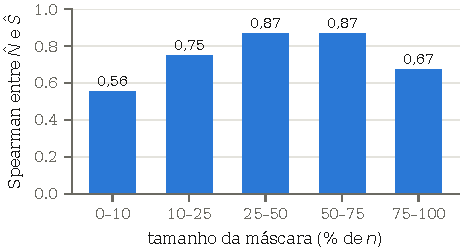
\includegraphics[width=\columnwidth]{correlacao}
\caption{Correlação de Spearman entre $\hat N$ e $\hat S$ entre máscaras de
mesmo tamanho, por faixa de tamanho relativo (média sobre as 99 instâncias).
Valores altos indicam que os dois objetivos ordenam as máscaras da mesma forma.}
\label{fig:correlacao}
\end{figure}

Os dois objetivos, portanto, não são redundantes na região de explicações
pequenas, e mantivemos os três. O conflito tem uma causa visível nas
probabilidades: entre máscaras de até 10 posições, os métodos de busca encontram
alguma com $\widehat{\PN}$ perto de 1, mas a melhor $\widehat{\PS}$ fica perto
de $0{,}55$ (Tabela~\ref{tab:metodos}). Poucos itens bastam para derrubar a
recomendação; poucos itens raramente bastam para sustentá-la contra um
histórico inteiro de itens neutros.

\subsection{Ajuste do NSGA-II}
\label{sec:ajuste}

Nos 30 usuários de ajuste, variamos a população em $\{25,50,100,200\}$ e $M$ em
$\{5,10,20\}$, sempre com $10^5$ passadas e 3 sementes
(Tabela~\ref{tab:ajuste}). Com o orçamento fixo, população e $M$ maiores
significam menos gerações, e o hipervolume cai nas duas direções. Escolhemos
população 25 e $M=10$. Ela é melhor que população 100 com $M=10$ em 27 dos 30
usuários ($p=3\times10^{-6}$ após Holm); a diferença para população 50 com
$M=10$ não é significativa ($p=0{,}23$). O \HVp{} quase não distingue as
configurações (entre $0{,}75$ e $0{,}78$, exceto $0{,}70$ na maior).

\begin{table}[t]
\caption{Ajuste do NSGA-II: hipervolume (todas as máscaras) nos 30 usuários de
ajuste, por tamanho da população e número de fundos $M$.}
\label{tab:ajuste}
\small
\begin{tabular}{@{}lccc@{}}
\toprule
População & $M=5$ & $M=10$ & $M=20$ \\
\midrule
\tabela{ajuste}
\bottomrule
\end{tabular}
\end{table}

\subsection{Comparação entre métodos}

\begin{table*}[t]
\caption{Comparação nas 99 instâncias, com frentes reavaliadas em $M'=100$
fundos independentes. \HVp{}: hipervolume das máscaras com até 10 posições; HV:
de todas as máscaras. Passadas: consultas ao SASRec usadas pela busca. PN e PS:
média da maior $\widehat{\PN}$ e da maior $\widehat{\PS}$ entre máscaras de até
10 posições.}
\label{tab:metodos}
\small
\begin{tabular}{@{}lcccrcc@{}}
\toprule
Método & \HVp & HV & Tamanho da frente & Passadas & PN & PS \\
\midrule
\tabela{metodos}
\bottomrule
\end{tabular}
\end{table*}

A Tabela~\ref{tab:metodos} resume a comparação. O quadro muda conforme a
região da frente.

\paragraph{Explicações pequenas.}
No \HVp{}, o NSGA-II é o melhor método. Ele supera o guloso em 71 das 99
instâncias ($p=1{,}8\times10^{-5}$ após Holm), o ranking por ablação em 89, o
GECE com reinícios em 96 e o AG escalarizado em 97 (todos com
$p<10^{-15}$). A diferença para o AG escalarizado, que usa os mesmos
operadores e o mesmo orçamento, é a mais informativa: dividir o orçamento
entre vetores de pesos cobre pior a região pequena do que uma única população
ordenada por dominância.

\paragraph{Todas as máscaras.}
No HV sem limite de tamanho a ordem se inverte: o guloso é o melhor e supera o
NSGA-II em 81 das 99 instâncias ($p=1{,}1\times10^{-9}$). O ranking por
ablação fica logo atrás usando 4\,615 passadas, menos de 5\% do orçamento. A
razão é estrutural: o guloso e o ranking percorrem todos os tamanhos de $1$ a
$n$, enquanto o NSGA-II, com inicialização esparsa, concentra a busca nas
máscaras pequenas. Como $\hat N$ e $\hat S$ concordam nas máscaras grandes
(Seção~\ref{sec:conflito}), ali uma ordenação simples das posições já basta.

\paragraph{Convergência.}
A Figura~\ref{fig:convergencia} mostra o \HVp{} ao longo da busca. O ranking
por ablação é o mais rápido no início e estaciona; o NSGA-II ultrapassa o
guloso depois de cerca de mil máscaras; o AG escalarizado só se aproxima no
fim, quando já rodou a maior parte dos seus vetores de pesos.

\begin{figure}[t]
\centering
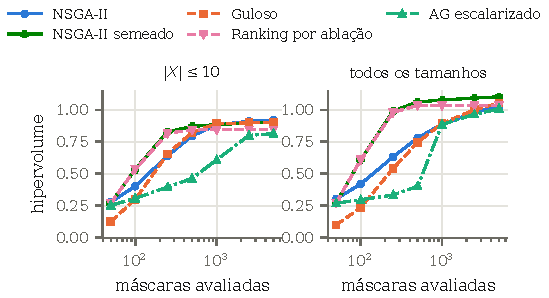
\includegraphics[width=\columnwidth]{convergencia}
\caption{\HVp{} em função do número de máscaras avaliadas (fundos de busca,
média sobre instâncias e sementes). O orçamento completo são 5\,000 máscaras.}
\label{fig:convergencia}
\end{figure}

\paragraph{Recência.}
Os itens escolhidos pelo NSGA-II em máscaras pequenas têm posição relativa
média de $0{,}84$: as explicações se concentram no fim do histórico, como o
GECE já havia observado~\cite{scarcelli2025gece}. Ainda assim, tomar apenas as
$k$ posições mais recentes rende \HVp{} de $0{,}755$, bem abaixo dos métodos
de busca: a recência indica onde procurar, mas não quais itens escolher. O
\HVp{} do NSGA-II varia pouco com a popularidade do alvo ($0{,}91$, $0{,}95$ e
$0{,}90$ nos tercis de baixa, média e alta popularidade).

\subsection{Operadores do NSGA-II}
\label{sec:operadores}

\begin{table}[t]
\caption{Estudo dos operadores do NSGA-II nos 30 usuários de ajuste. Cada
linha muda um único elemento da configuração ajustada.}
\label{tab:operadores}
\small
\begin{tabular}{@{}lccc@{}}
\toprule
Variante & \HVp & HV & Frente \\
\midrule
\tabela{operadores}
\bottomrule
\end{tabular}
\end{table}

A Tabela~\ref{tab:operadores} isola cada escolha. A inicialização esparsa é a
que mais importa: com inicialização uniforme (metade dos bits ligados), o
\HVp{} cai de $0{,}911$ para $0{,}478$, porque a busca gasta o orçamento
descendo de máscaras grandes. Retirar o cruzamento custa cerca de $0{,}10$ de
\HVp{} e quase nada de HV. A taxa de mutação é um compromisso: $0{,}5/n$ ganha
um pouco nas máscaras pequenas (melhor em 23 de 30 usuários, $p=0{,}003$) e
perde no HV geral (pior em 26 de 30); taxas maiores pioram os dois. Mantivemos
$1/n$.

\subsection{Verificação contra a frente exata}
\label{sec:exata}

Nos históricos do experimento, a frente verdadeira é desconhecida. Todo
usuário do MovieLens-20M tem ao menos 19 itens antes do item de teste, de modo
que nenhum histórico real é curto o bastante para ser enumerado. Para medir o
quanto o NSGA-II se aproxima da frente exata, usamos como histórico apenas os
12 itens mais recentes de 20 usuários, com os mesmos candidatos, a mesma regra
de sorteio do alvo e os mesmos fundos. Isso deixa $2^{12}-1=4\,095$ máscaras
por instância, todas avaliadas; a frente exata tem em média 30 máscaras.

\begin{table}[t]
\caption{NSGA-II e busca aleatória contra a frente exata em 20 históricos de
12 itens (5 sementes). HV: fração do hipervolume da frente exata; Frente:
fração das máscaras da frente exata encontradas.}
\label{tab:exata}
\small
\begin{tabular}{@{}rrcccc@{}}
\toprule
 & & \multicolumn{2}{c}{NSGA-II} & \multicolumn{2}{c}{Aleatório} \\
\cmidrule(lr){3-4}\cmidrule(l){5-6}
Máscaras & \% do espaço & HV (\%) & Frente (\%) & HV (\%) & Frente (\%) \\
\midrule
\tabela{exata}
\bottomrule
\end{tabular}
\end{table}

A Tabela~\ref{tab:exata} mostra o resultado. Com 500 máscaras (12\% do
espaço), o NSGA-II atinge $99{,}5\%$ do hipervolume exato e encontra 89\% das
máscaras da frente; com 1\,000, praticamente a frente inteira. A busca
aleatória com as mesmas 1\,000 máscaras encontra 42\% da frente. Em históricos
enumeráveis, portanto, o NSGA-II converge para a frente exata com uma fração
pequena do espaço. Nada garante o mesmo com $n$ até 128, em que o orçamento
cobre uma fração ínfima de $2^n$.

\subsection{AG escalarizado e GECE}

\paragraph{Ajuste do AG escalarizado.}
Para que a comparação não dependa de uma configuração ruim da linha de base,
variamos sua população em $\{10,25,50\}$ e o número de vetores de pesos em
$\{6,10,15\}$ nos usuários de ajuste (Tabela~\ref{tab:escalar}). Nenhuma
configuração vence nos dois critérios: populações pequenas com poucos vetores
têm o maior HV (até $0{,}974$), e as intermediárias o maior \HVp{}. A
configuração usada na comparação principal (população 20, 10 vetores) fica
entre duas que empatam estatisticamente com a melhor em um dos critérios, e a
variação de \HVp{} entre configurações vizinhas é bem menor que a distância
para o NSGA-II na Tabela~\ref{tab:metodos}.

\begin{table}[t]
\caption{Ajuste do AG escalarizado: \HVp{} nos 30 usuários de ajuste, por
população e número de vetores de pesos.}
\label{tab:escalar}
\small
\begin{tabular}{@{}lccc@{}}
\toprule
População & 6 vetores & 10 vetores & 15 vetores \\
\midrule
\tabela{escalar-pequenas}
\bottomrule
\end{tabular}
\end{table}

\paragraph{GECE.}
Como distribuído no TRACE, o GECE sempre encontra um contrafactual válido (495
de 495 execuções) e para depois de 281 consultas em média; com tão poucas
máscaras avaliadas, sua frente fica entre as piores. Com reinícios até o orçamento
completo, ele sobe para perto da linha de base de recência e continua abaixo do
AG escalarizado sobre máscaras. A resposta que o GECE devolve muda uma única
posição em 73\% das execuções. Avaliadas com fundos novos, essas posições têm
$\widehat{\PN}$ média de $0{,}43$, e só 43\% delas são necessárias pelo nosso
critério ($\widehat{\PN}>0{,}5$). Em mais da metade dos casos, portanto, o
contrafactual do GECE depende do item específico que ele inseriu, e não da
posição editada. Isso não é um defeito do GECE, que responde a outra pergunta
(``que edição muda a recomendação?''); mostra que as duas formulações não são
intercambiáveis.

\subsection{Ablações da distribuição de fundo}
\label{sec:ablacao}

Repetimos a busca com dois outros preenchimentos: trechos contíguos do
histórico de outros usuários, mais plausíveis que itens independentes, e
\emph{padding}, em que as posições são simplesmente removidas. Em ambos os
casos as frentes são reavaliadas com os fundos de popularidade da comparação
principal: a pergunta é se explicações encontradas com outro preenchimento
continuam boas (Tabela~\ref{tab:ablacao}).

\begin{table}[t]
\caption{Ablação do preenchimento usado na busca. Todas as frentes são
reavaliadas com fundos de popularidade.}
\label{tab:ablacao}
\small
\begin{tabular}{@{}llcc@{}}
\toprule
Método & Preenchimento na busca & \HVp & HV \\
\midrule
\tabela{ablacao}
\bottomrule
\end{tabular}
\end{table}

Com trechos de outros usuários, os resultados se mantêm: as frentes são tão
boas quanto as da busca original ou ligeiramente melhores, e a ordem dos
métodos na região pequena é a mesma. Com \emph{padding}, todos os métodos
pioram em cerca de 90 das 99 instâncias. Explicações encontradas removendo
itens não se transferem para a substituição: remover desloca a sequência e
muda as posições de todos os itens anteriores, o que é uma intervenção
diferente. As posições escolhidas confirmam a leitura: a similaridade do
cosseno entre as frequências de seleção de cada posição é $0{,}99$ entre
sementes da busca original, $0{,}88$ entre a original e a de outros usuários,
e $0{,}72$ entre a original e a de \emph{padding}.

\subsection{Um exemplo}

\begin{table}[t]
\caption{Uma explicação de quatro itens para a recomendação de \emph{Full
Metal Jacket (1987)} a um usuário com histórico de 40 filmes
($\widehat{\PN}=0{,}97$, $\widehat{\PS}=0{,}86$). A posição 40 é a mais
recente.}
\label{tab:exemplo}
\small
\begin{tabular}{@{}rl@{}}
\toprule
Posição & Filme \\
\midrule
\tabela{exemplo}
\bottomrule
\end{tabular}
\end{table}

\begin{figure}[t]
\centering
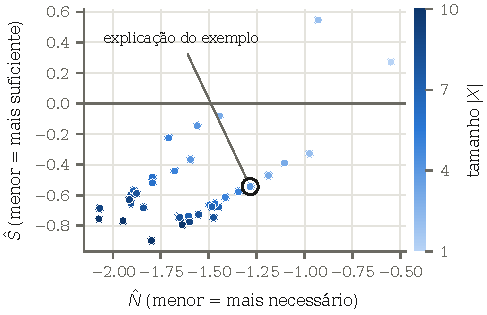
\includegraphics[width=\columnwidth]{exemplo-frente}
\caption{Frente do NSGA-II para a instância da Tabela~\ref{tab:exemplo}
(máscaras de até 10 posições, uma semente). O círculo marca a explicação da
tabela.}
\label{fig:exemplo}
\end{figure}

A Tabela~\ref{tab:exemplo} mostra uma explicação da frente do NSGA-II.
Substituir esses quatro filmes tira \emph{Full Metal Jacket} do top-10 em 97\%
dos fundos, e mantê-los sozinhos o sustenta em 86\%. A melhor explicação de um
único item (o filme mais recente, \emph{Reservoir Dogs}) é necessária em 75\%
dos fundos, mas suficiente em apenas 40\%. A Figura~\ref{fig:exemplo} mostra o
que uma resposta única esconderia: o usuário da explicação pode trocar tamanho
por força, e as máscaras maiores avançam nos dois objetivos ao mesmo tempo.
